
\chapter{Conclusiones y mejoras}

\section{Seguridad}

\setlength{\parindent}{5ex}Después de Utilizar Arduino he podido apreciar que es bastante bueno para el aprendizaje pero para una aplicación real deja mucho que desear ya que en un entorno educacional si se produce algún error se puede corregir en el momento y estos no serán provocados, ademas debido a la incapacidad nativa del SAM3X para encirptar la informacion, en este caso pretendía realizar peticiones HTTPS al servidor, el sistema es muy debil a ataques MitM (\textit{Man-in-the-middle}) pues la informacion que envía no esta encirptada de ningún modo ni existe algún tipo de bloqueo a peticiones externas que no tengan nada que ver con la aplicación por lo que esto queda muy lejos de ser una aplicación final pues se puede romper por este hueco de seguridad.

\setlength{\parindent}{0ex}\textit{Un ataque man-in-the-middle es un ataque en el que se adquiere la capacidad de leer, insertar y modificar a voluntad, los mensajes entre dos partes sin que ninguna de ellas conozca que el enlace entre ellos ha sido violado. El atacante debe ser capaz de observar e interceptar mensajes entre las dos víctimas.}\cite{mitm}.

Para solucionar esto, he pensado en utilizar controladoras que permitan encriptación o conexión SSH lo cual requeriría un rendimiento mayor y un mayor consumo, o también, la aplicación solo pueda estar disponible para una red interna, lo que la limitaría a un área muy reducida ya que si esta conectada a Internet, el área de alcance es a nivel global pero insegura, por lo que resolviendo algunos problemas surgen otros nuevos.

\section{Sensores}

\setlength{\parindent}{5ex}He tenido aprendizaje en el funcionamiento de la electrónica básica ha sido gracias a los diversos problemas entre versiones de Arduino y los cambios realizados en los circuitos para poder implementarlos.
\setlength{\parindent}{0ex}
Ademas de otros problemas, los sensores no dan siempre un valor fiable, en el proyecto los he tratado como valores anómalos, los cuales son valores que no corresponden con lo que deberían de dar ya sea por error de lectura o fallo de los componentes debido a su montaje en cableado.

Para poder solucionar esto habría que tener en cuenta 2 casos:

\begin{itemize}
	\item \textbf{Circuito:} Todo esto podría mejorar si en vez de implementa el circuito en una \textit{protoboard} se habría creado un circuito impreso y soldado los componentes directamente a la placa y estos pines conectarlos al Arduino con el fin de suprimir la \textit{protoboard}, cables y componentes de electrónica básica que permiten funcionar correctamente los sensores. Esto suprimiría los errores de fallos de conexión o cortocircuitos en la aplicación ademas de reducir notablemente el tamaño del nodo.   
	
	\item \textbf{Sensores} Los sensores que he utilizado para el proyecto son de un coste reducido, por ejemplo, hay sensores que durante el montaje de este proyecto se han quemado, no son para una larga duración, debido a su coste y tampoco son muy exactos, para solucionar esto se deberían implementar sensores mas eficientes de un coste mas elevado, por ejemplo reemplazar el DHT11 de unos 2\euro por su versión mas cara el DHT33 por 17\euro.

\end{itemize}

\section{Boards especializadas}

\setlength{\parindent}{5ex}Analizando en este proyecto lo que he podido obtener de informacion sobre Arduino es que no sirve mucho para realizar este tipo de funciones, como se ha descrito anteriormente solo sirve para el ámbito educacional y demás, sin embargo todo este sistema ya existe a nivel comercial, así que analizando en Internet he obtenido informacion sobre una controladora que, ofrezca la informacion segura y que permita conectarse por una red, tanto cableada como inalámbrica (incluyendo GPRS) y que tenga un consumo muy reducido.
\setlength{\parindent}{0ex}
Se trata de la controladora FlyPort que en cierta medida soluciona los problemas que se han descrito anteriormente sin embargo lejos de ser la panacea el problema es que al ser comercial su precio es muy elevado ya que aunque la controladora sea barata, requiere de un sistema para poder implementar los sensores y poder programarla.

En la \textbf{Figura \ref{fig:flyportimg}} esta la imagen del \textit{Started kit} de la controladora en cuestión: 

\begin{figure}[!h]
	\centering
	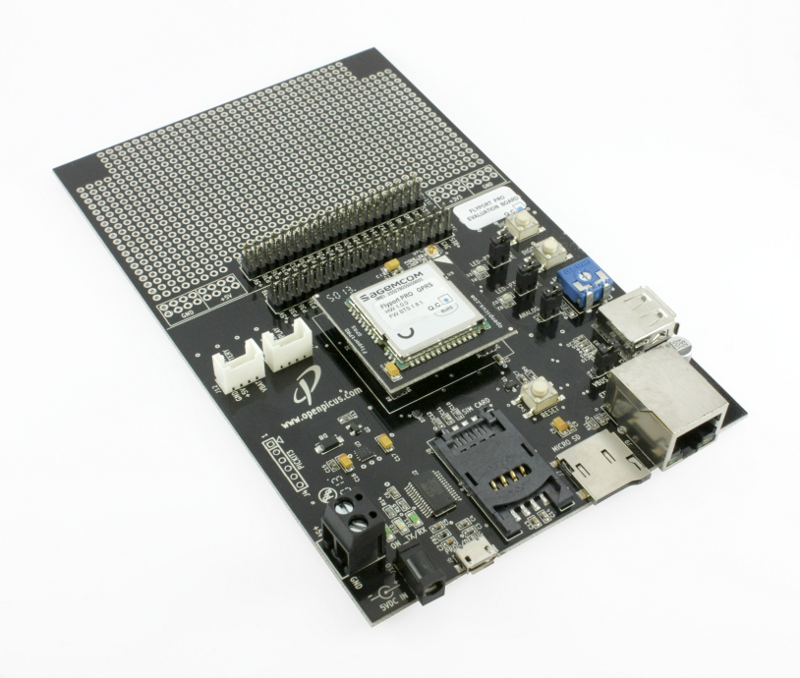
\includegraphics[width=0.5\linewidth]{figuras/flyportimg}
	\caption{FlyPort GPRS y la placa para la controladora.\cite{FlyPort}}
	\label{fig:flyportimg}
\end{figure}

El coste de este \textit{Started kit} es de unos 150\euro aproximadamente y como he hablado en la sección anterior también se va a añadir el coste de sensores de calidad al nodo, teniendo en cuenta que al ser de calidad son de un coste mucho mas caro que los que he utilizado para este proyecto, el coste puede subir perfectamente a los 200\euro

